\subsection{Agent Function Architecture}\label{subsec:AgentFNArch}
%\note{This section shows how the agent function is implemented. Diagram shows how DerivedOccupancyGridAgent actually operates.}
Putting together the components outlined so far in this chapter, we end up with an agent function that is shown in Figure \ref{fig:BasicAgentArchitecture}. 

\note{Fix this figure}
\begin{figure}[H]
    \centering
    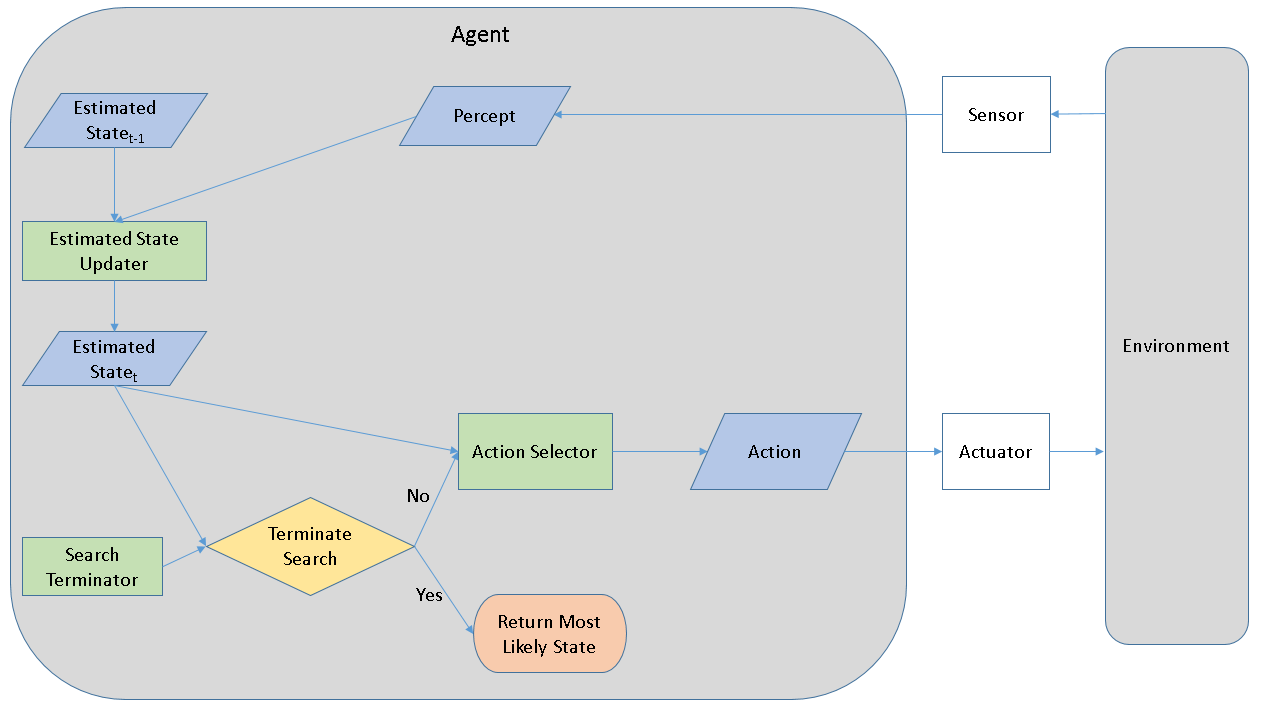
\includegraphics[width = 0.8\linewidth]{Chapters/MultiAgentTargetDetection/Figs/AgentFnArchitecture/BasicAgentFunctionNoCommunication.PNG}
    \caption{The structure of the agent function.}
    \label{fig:BasicAgentArchitecture}
\end{figure}


The diagram outlines how the agent interacts with its environment and abstracts away technical details such as the search status. This is a concrete version of the model-based reflex agent outlined in \cite[P~.51]{AIAMA}. The estimated state update rules are applied as outlined in the previous sections in this chapter. Algorithm \ref{alg:SingleTargetLocalisation} shows the algorithm which describes the agent function.
\note{might be able to bulk this up a bit, come back to it}



\begin{algorithm}[H]
\caption{Single Target Localisation Algorithm}
\label{alg:SingleTargetLocalisation}

\begin{algorithmic}[1]
\renewcommand{\algorithmicrequire}{\textbf{Input:}}
\renewcommand{\algorithmicensure}{\textbf{Output:}}
%Input
\REQUIRE $ \newline initial\_estimated\_state = P(x_{0} | e_{0}, u_0), \quad \text{ The initial distribution of the estimated state}
\newline select\_action, \quad \text{Returns an action given an estimated state}
\newline estimated\_state\_updater, \quad \text{Returns the updated estimated state given the current} \newline \text{ estimated state, a percept and an action}
\newline SPRT, \quad \text{An object calibrated with a specified Type \Romannum{1}, Type \Romannum{2} error which has a } \newline \text{method to implement the SPRT and an attribute which returns the result of the}
\newline
\text{application of the SPRT.}
$
%Output
\ENSURE  $\newline \text{The grid cell containing the source, } x_i \text{ for } i \in \{1, ..., N\}, \text{ or } x_{N+1} \text{, indicating} \newline \text{ the source is not present}$

\hfill\pagebreak

\STATE $estimated\_state$ $\leftarrow$ $initial\_estimated\_state$
\WHILE{not $SPRT.should\_terminate\_search(estimated\_state)$}
\STATE $action \leftarrow select\_action(estimated\_state)$
\STATE $perform\_action(action)$
\STATE $percept \leftarrow get\_percept()$
\STATE $estimated\_state \leftarrow estimated\_state\_updater(estimated\_state, percept, action)$
\ENDWHILE
\RETURN $\argmax_{x_i}{p(x_i | e_{1:t}, u_{1:t}) = \argmax estimated\_state}$
\end{algorithmic} 
\end{algorithm}